% Generated by management.py report; do not edit.
\setlength{\tabcolsep}{2pt}
\begin{tabular}{ccc}
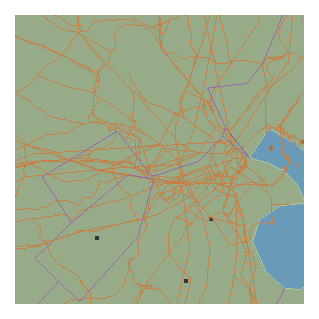
\includegraphics[width=0.31\textwidth]{figures/analysis_sample_natural_earth_vector.pdf} & 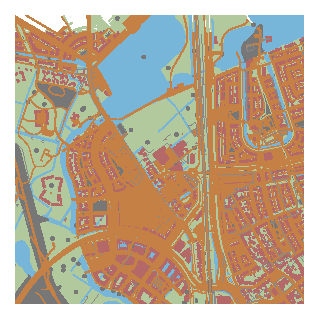
\includegraphics[width=0.31\textwidth]{figures/analysis_sample_pdok_netherlands_infrostructure.pdf} & 
\includegraphics[width=0.31\textwidth]{figures/analysis_sample_usfws_luisiana_wetlands_geopackage.pdf} \\
\shortstack{(a) Natural Earth\\\scriptsize $z=11$, $x=619$, $y=757$} & \shortstack{(b) PDOK BGT\\\scriptsize $z=14$, $x=8458$, $y=5421$} & \shortstack{(c) USFWS\\\scriptsize $z=14$, $x=4092$, $y=6789$} \\[4pt]

\includegraphics[width=0.31\textwidth]{figures/analysis_sample_swisstopo_mountains_vector.pdf} & 
\includegraphics[width=0.31\textwidth]{figures/analysis_sample_louisiana-260912.pdf} &  \\
\shortstack{(d) swisstopo\\\scriptsize $z=14$, $x=8623$, $y=5743$} & \shortstack{(e) OSM\\\scriptsize $z=14$, $x=4092$, $y=6791$} &  \\[4pt]
\end{tabular}
\par\smallskip
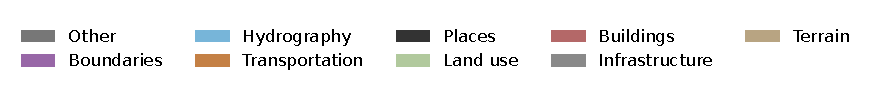
\includegraphics[width=0.85\textwidth]{figures/analysis_sample_legend.pdf}
\caption{Samples decoded from Standard MVT tiles with a common style based on retained tile-layer names.
Each panel selects the tile with the most vertices at the highest stored zoom; addresses are shown below the panels.
Colours denote layer names and do not reclassify their contents. Sources: Natural Earth / NACIS; Source: PDOK; U.S. Fish and Wildlife Service, National Wetlands Inventory; Source: swisstopo; \copyright{} OpenStreetMap contributors, ODbL.}
